\begin{figure}[htbp]
    \centering
    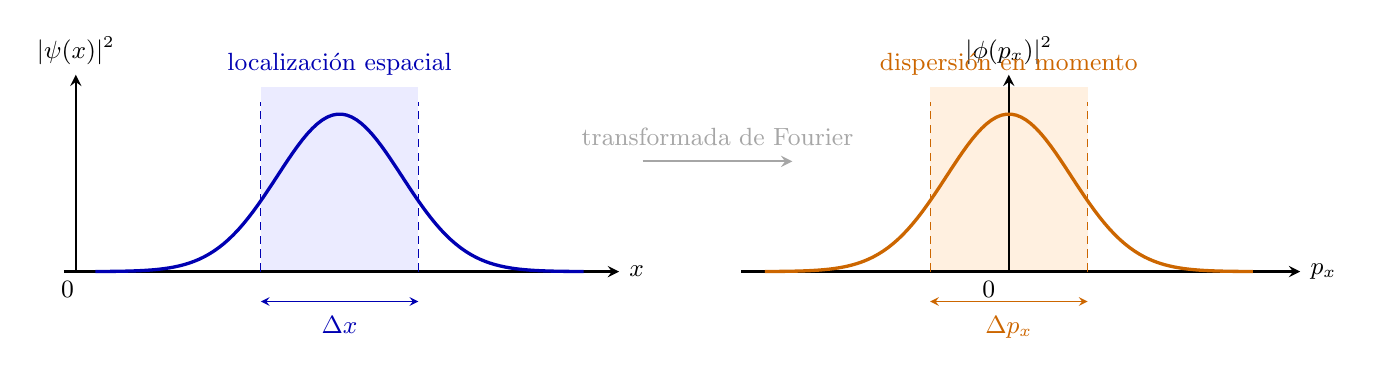
\begin{tikzpicture}[>=stealth, every node/.style={font=\small}]
        \fill[blue!8] (-1,0) rectangle (1,2.35);
        \draw[->,thick] (-3.5,0) -- (3.55,0) node[right] {$x$};
        \draw[->,thick] (-3.35,0) -- (-3.35,2.5) node[above] {$|\psi(x)|^2$};
        \draw[densely dashed,blue!70!black] (-1,0) -- (-1,2.15);
        \draw[densely dashed,blue!70!black] (1,0) -- (1,2.15);
        \draw[very thick,blue!70!black,domain=-3.1:3.1,samples=100]
            plot (\x,{2.0*exp(-0.8*\x*\x)});
        \draw[<->,blue!70!black] (-1,-0.38) -- (1,-0.38)
            node[midway,below=2pt] {$\Delta x$};
        \node[blue!70!black,above] at (0,2.37) {localización espacial};
        \node[below left] at (-3.25,0) {$0$};

        \fill[orange!12] (7.5,0) rectangle (9.5,2.35);
        \draw[->,thick] (5.1,0) -- (12.2,0) node[right] {$p_x$};
        \draw[->,thick] (8.5,0) -- (8.5,2.5) node[above] {$|\phi(p_x)|^2$};
        \draw[densely dashed,orange!80!black] (7.5,0) -- (7.5,2.15);
        \draw[densely dashed,orange!80!black] (9.5,0) -- (9.5,2.15);
        \draw[very thick,orange!80!black,domain=-3.1:3.1,samples=100]
            plot ({8.5+\x},{2.0*exp(-0.8*\x*\x)});
        \draw[<->,orange!80!black] (7.5,-0.38) -- (9.5,-0.38)
            node[midway,below=2pt] {$\Delta p_x$};
        \node[orange!80!black,above] at (8.5,2.37) {dispersión en momento};
        \node[below left] at (8.45,0) {$0$};

        \draw[->,gray!70,thick] (3.85,1.4) -- (5.75,1.4)
            node[midway,above=2pt] {transformada de Fourier};
    \end{tikzpicture}
    \caption{Esquema de la relación entre la localización de un paquete de onda y su distribución de momentos. Las curvas son ilustrativas; al reducir $\Delta x$ aumenta la dispersión $\Delta p_x$, de acuerdo con $\Delta x\,\Delta p_x\geq\hbar/2$.}
    \label{fig:incertidumbre}
\end{figure}